\documentclass[border=10pt]{standalone}
\usepackage[svgnames]{xcolor}
\usepackage{amsmath}
\usepackage{pgfplots}
\pgfplotsset{compat=newest}
\usepackage[sfdefault]{FiraSans}
\usepackage{FiraMono}
\renewcommand*\familydefault{\sfdefault}
\begin{document}
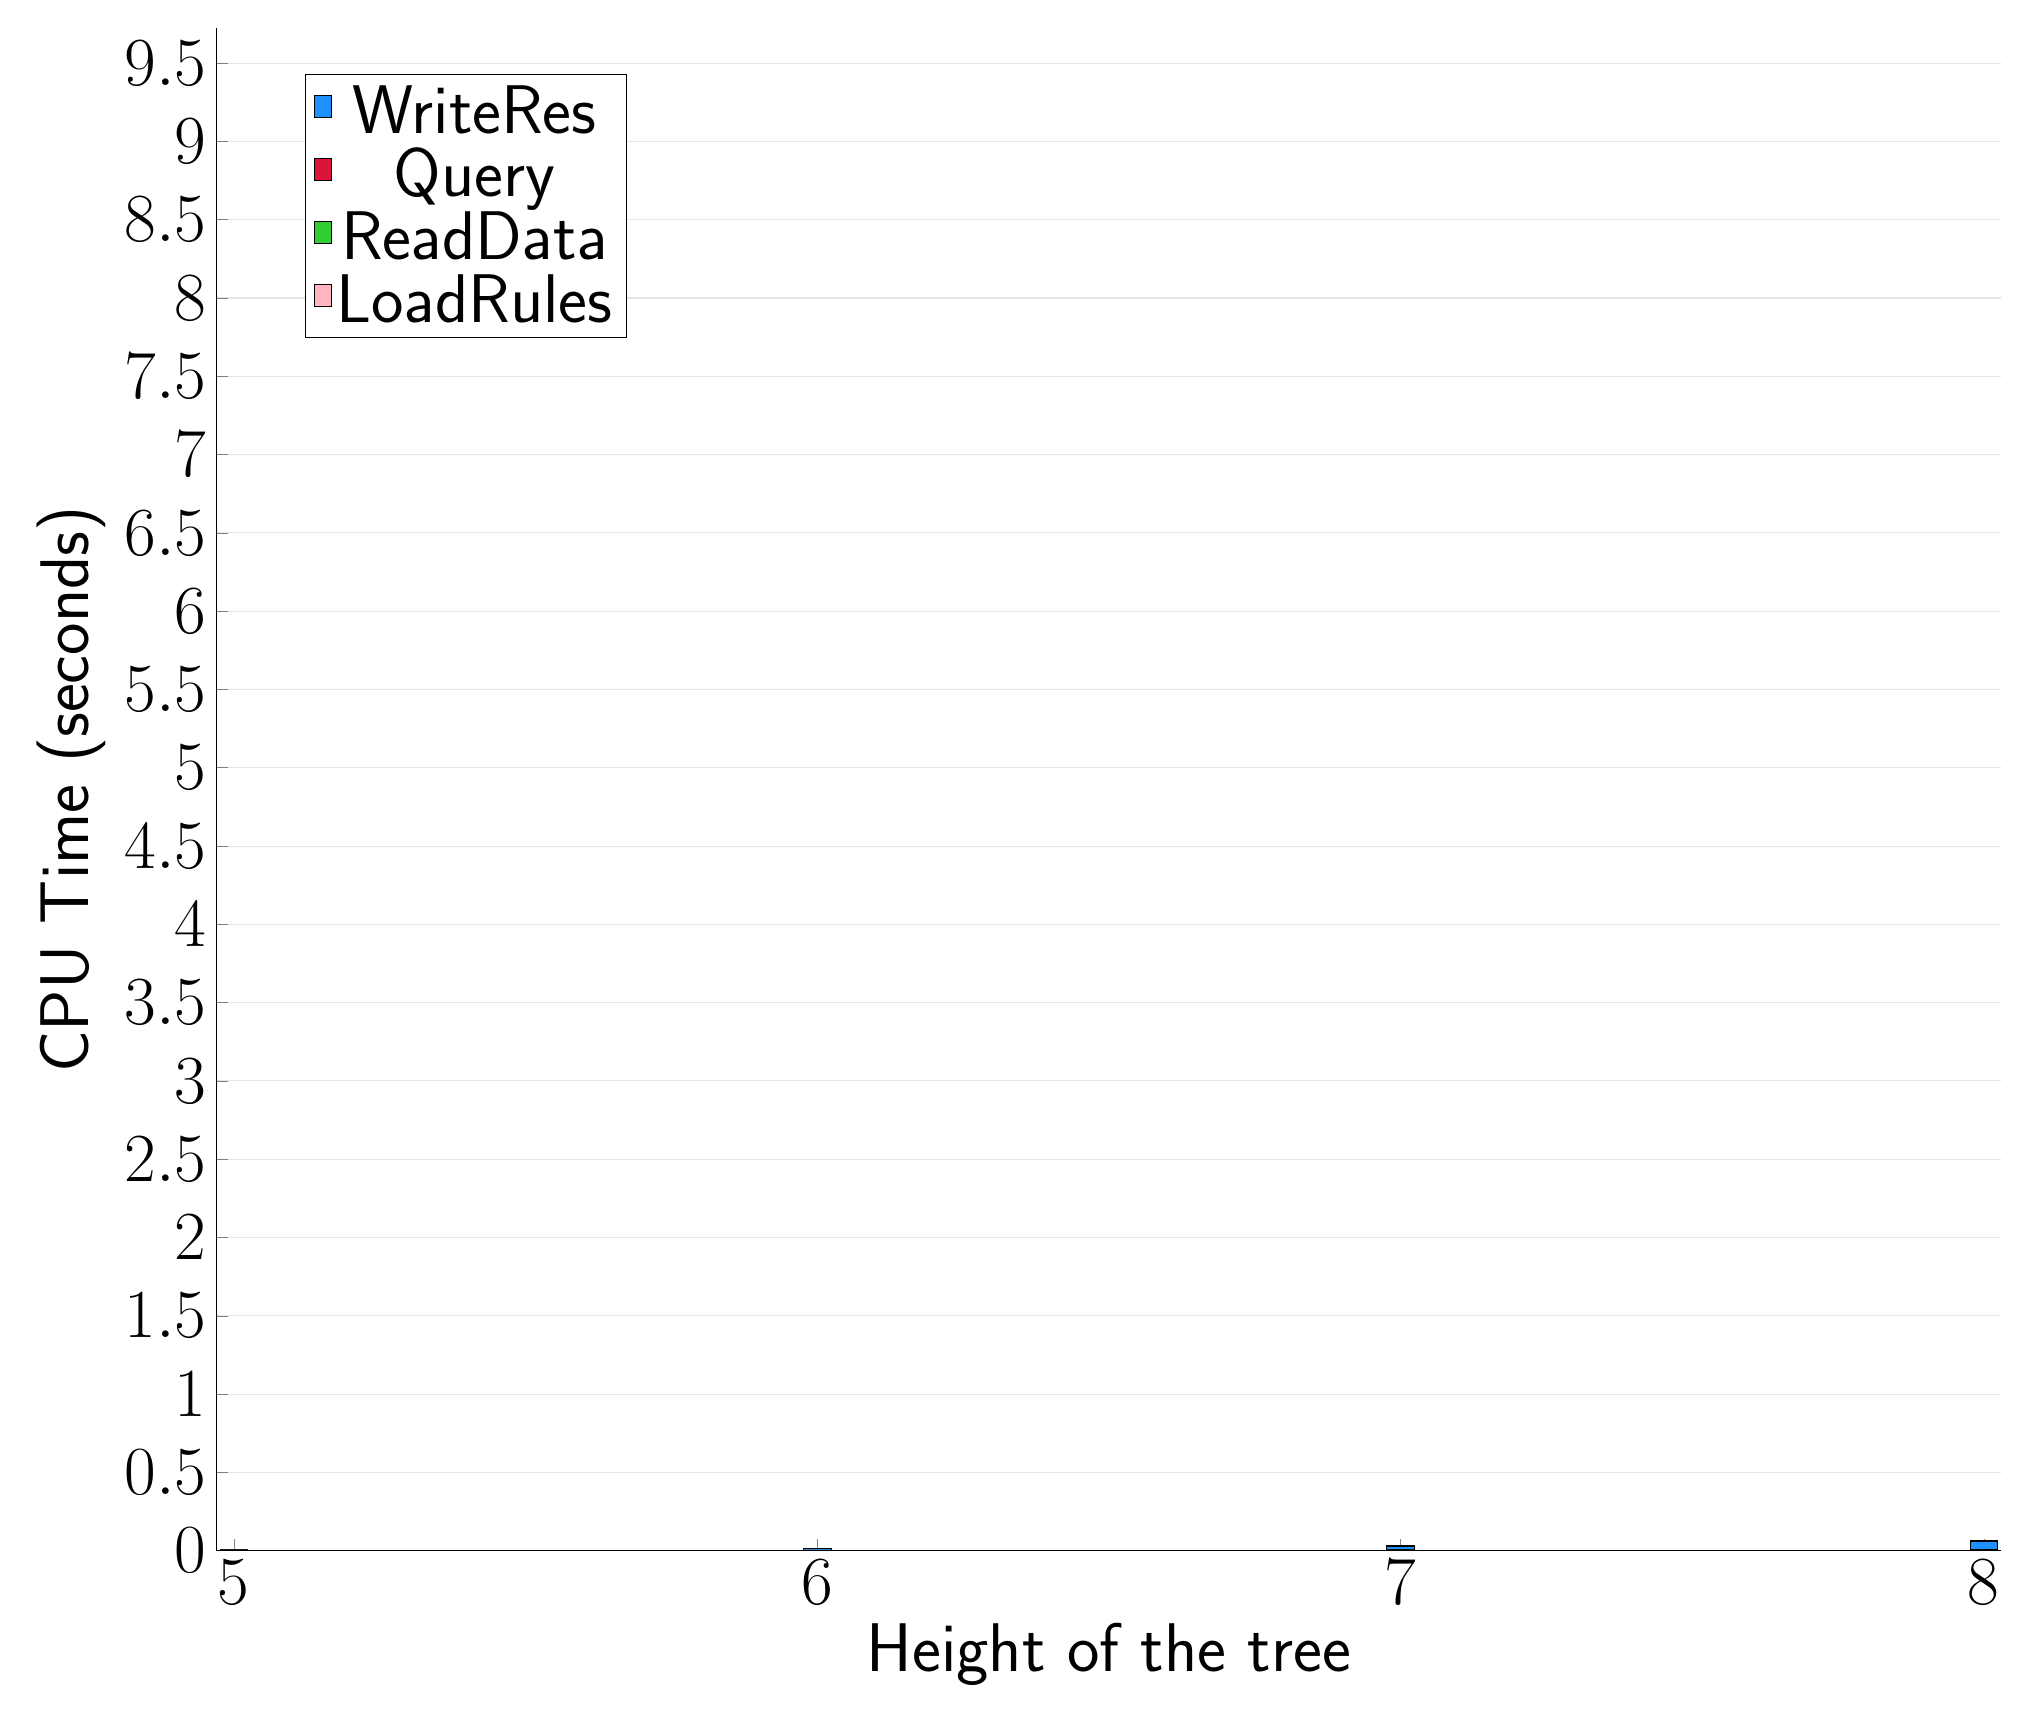
\begin{tikzpicture}
\begin{axis}[
   ybar stacked,
   width=2\textwidth,
   bar width=0.35cm,
   ymajorgrids, tick align=inside,
   major grid style={draw=gray!20},
   xtick=data,
   ymin=0, ymax=9.723333331445852,
   axis x line*=bottom,
   axis y line*=left,
   enlarge x limits=0.01,
   legend style={
       at={(0.23, 0.97)},
       anchor=north east,
       legend columns=1,
       font=\Huge,
   },
   ylabel={CPU Time (seconds)},
   xlabel={Height of the tree},
   label style={font=\Huge},
   tick label style={font=\Huge},
]
\addlegendimage{fill=DodgerBlue, draw=black, line width=0.2pt}
\addlegendentry{WriteRes}
\addlegendimage{fill=Crimson, draw=black, line width=0.2pt}
\addlegendentry{Query}
\addlegendimage{fill=LimeGreen, draw=black, line width=0.2pt}
\addlegendentry{ReadData}
\addlegendimage{fill=LightPink, draw=black, line width=0.2pt}
\addlegendentry{LoadRules}
\addplot +[fill=LightPink, draw=black, line width=0.2pt] coordinates {
(5, 0.0033443333333333333)
(6, 0.0036093333333333338)
(7, 0.0014883333333333335)
(7, 0.003356333333333333)
(7, 0.003124333333333333)
(8, 0.0037563333333333303)
(8, 0.0032073333333333333)
(8, 0.004022666666666663)
};
\addplot +[fill=LimeGreen, draw=black, line width=0.2pt] coordinates {
(5, 0.0010013333333333341)
(6, 0.0013993333333333334)
(7, 0.0016370000000000002)
(7, 0.0020286666666666634)
(7, 0.0018419999999999999)
(8, 0.0037633333333333334)
(8, 0.0038220000000000003)
(8, 0.0042309999999999995)
};
\addplot +[fill=Crimson, draw=black, line width=0.2pt] coordinates {
(5, 5.2333333333334766e-05)
(6, 0.00013566666666666363)
(7, 0.00012766666666666701)
(7, 0.000217666666666667)
(7, 0.00021700000000000167)
(8, 0.0005273333333333333)
(8, 0.0007116666666666683)
(8, 0.0006200000000000027)
};
\addplot +[fill=DodgerBlue, draw=black, line width=0.2pt] coordinates {
(5, 0.004448999999999998)
(6, 0.010534333333333335)
(7, 0.024505)
(7, 0.023188333333333328)
(7, 0.02675633333333333)
(8, 0.05370666666666666)
(8, 0.056115)
(8, 0.056848333333333334)
};
\end{axis}
\end{tikzpicture}

\end{document}
